\section{Health Types}
After the K-means clustering algorithm assigned four distinct clusters to the eligible individuals aged 50--60, I observed the following heterogeneity in health trajectories. My analysis revealed three distinct health types, each characterized by different patterns of frailty progression and mortality risks.

The analysis revealed a striking disparity in the distribution of health types within the sample population. Type~I emerged as the dominant trajectory, accounting for 91.7\% of the sample, while Types~II and III represented only 3.9\% and 4.4\%, respectively. This marked imbalance suggests the presence of distinct underlying characteristics or risk factors associated with the less common health trajectories, warranting further investigation. Table~\ref{tab:type_dist} summarizes the distribution.

\begin{table}[ht]
    \centering
    \caption{Health type distribution in the clustering sample}
    \label{tab:type_dist}
    \begin{tabular}{lrr}
        \toprule
        Health Type & Share of Sample (\%) & Description \\
        \midrule
        Type I & 91.7 & Resilient health type \\
        Type II & 3.9 & Early onset frailty type \\
        Type III & 4.4 & Accelerated decline type \\
        \bottomrule
    \end{tabular}
\end{table}


At age 40, the starting point of the data, I observed a growing divergence in frailty profiles across types. These trajectories can be summarized as follows:
\begin{itemize}
    \item \textbf{Type I (Resilient Health Type).} Starts with the lowest frailty and shows a very gradual, steady increase over time, maintaining the lowest frailty index throughout the entire age range. This type represents the majority of the population.
    \item \textbf{Type II (Early Onset Frailty Type).} Begins with the highest initial frailty and experiences a more pronounced increase, especially after age 60.
    \item \textbf{Type III (Accelerated Decline Type).} Starts between Types I and II but rapidly increases, surpassing Type II around age 55. It shows some fluctuations but generally maintains higher frailty levels in later years.
\end{itemize}

These distinct trajectories highlight the heterogeneity in health patterns across the population and underscore the importance of considering these differences in health and economic analyses. By age 70, I observe a widening gap between the ``resilient health type'' and the other two types. This suggests that initial health trajectories can significantly influence long-term health outcomes, at least when considering these specific health deficits.

\begin{figure}[ht]
    \centering
    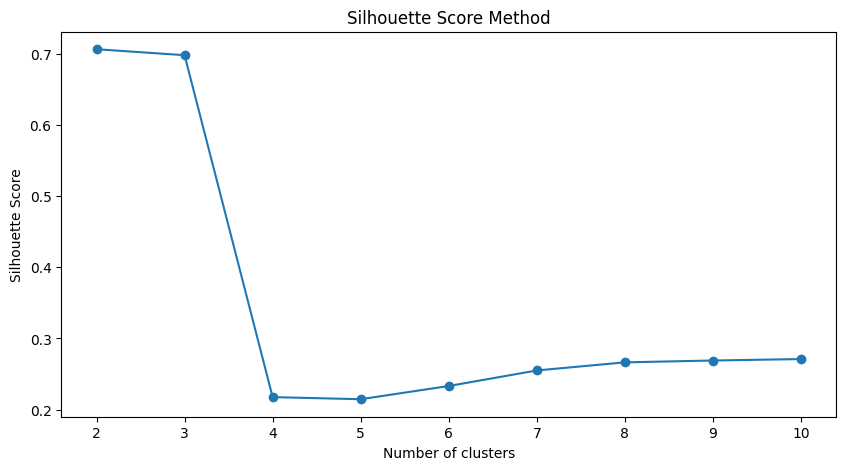
\includegraphics[width=0.85\textwidth]{figures/fig-009.png}
    \caption{Frailty trajectories by health type (extracted from the original dissertation PDF).}
    \label{fig:health_types}
\end{figure}
